\section{Preliminary Models}
\subsection{Daimler Models}

\subsubsection*{Introduction}

The basic settings of the DAIMLER's use-case \cite{Fer14}	 are as follows. Let us suppose we are driving our car, which will be referred as the EGO vehicle, in a highway. This EGO vehicle is equipped with a video camera, radar and some on-board sensors.  Using the data provided by these sensors, the challenge consists in the early recognition of a manoeuvre either of the EGO or another relevant car in the traffic scene (OBJ). In total, the system is expected to recognised the following set of manoeuvres (a visual description of them is given below in Figure \ref{Figure:DaimlerManeuvers}):
\begin{enumerate}
\item \textbf{Object-CutOut}:  A vehicle that was driving in front of us is leaving the EGO lane.
\item \textbf{Object-CutIn}: A vehicle is moving to the lane where the EGO vehicle is placed.
\item \textbf{EGO-CutOut}: The EGO vehicle is leaving the lane where it was driving.
\item \textbf{EGO-CutIn}: The EGO vehicle is moving to a new lane already occupied by another vehicle. 
\item \textbf{Object-Follow}: There is no lane change. The EGO is driving and there is some other vehicle in front.
\item \textbf{Lane-Follow}: There is no lane change. The EGO is driving and there is not any other vehicle in front.
\end{enumerate}

\begin{figure}
\begin{center}
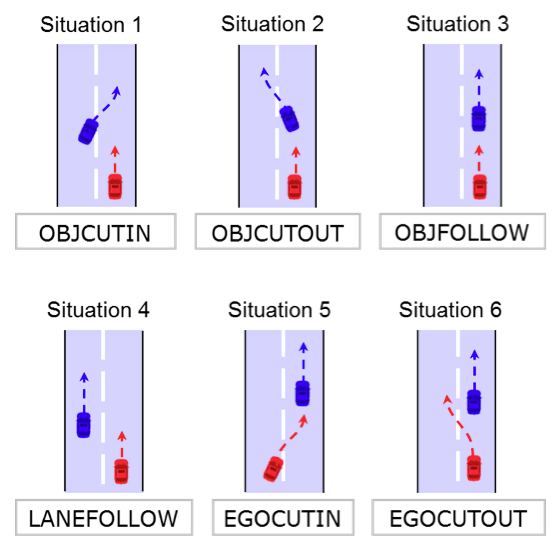
\includegraphics[scale=0.4]{./figures/DaimlerManeuvers}
\caption{\label{Figure:DaimlerManeuvers}Different maneuvers which should be identified by the AMIDST system.  Red blocks represents the EGO vehicle and blue blocks represents other vehicles in the scene. In the first four maneuvers, there is a lane change event or, under Daimler's terminology, a ``Lane Marking Crossing'' (LMC) event. 
}
\end{center}
\end{figure}

Instead of working with the raw data from the video, radar and on-board sensors, the manoeuvre recognition system uses the so-called ``object data'', which contains ``high level'' representations or features describing the ``traffic scene'' such as EGO's speed, distance between EGO and another vehicle in front, etc.  
\begin{figure}
\begin{center}
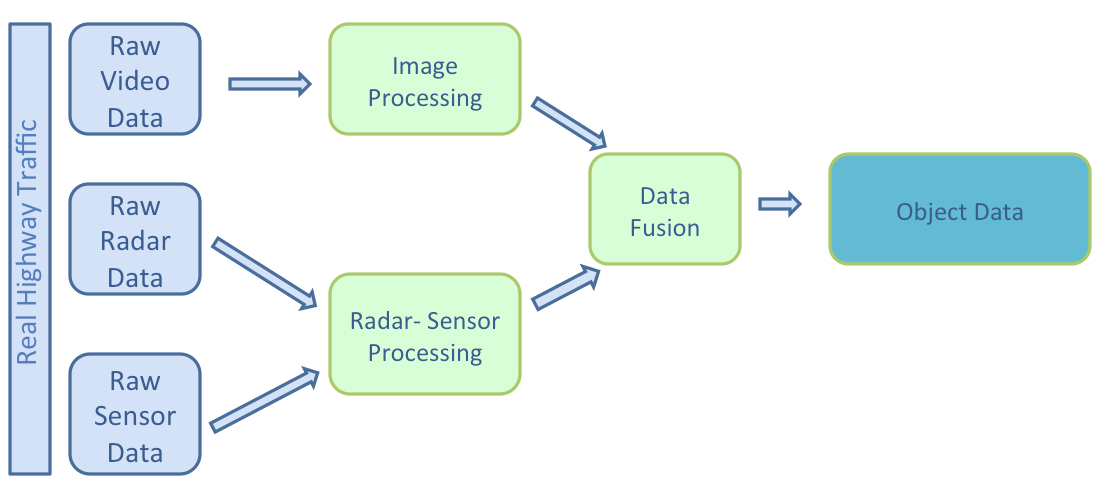
\includegraphics[scale=0.35]{./figures/DaimlerDataFlow}
\caption{\label{Figure:DaimlerDataFlow} Daimler's Data Flow.}
\end{center}
\end{figure}

Figure \ref{Figure:DaimlerDataFlow} contains a visual description of the current data flow used to create this ``object data''.  As can be seen in this figure, in a first step the raw data coming from the video, radar and sensors is preprocessed. In a second step this preprocessed data is fused and the high-level or ``object data'' describing the traffic scene is obtained. 

Using the resulting ``object data'', Daimler has developed a probabilistic graphical model \cite{kasper2012object} which is able to recognize an ongoing manoeuvre around 0.6 seconds before the manoeuvre really takes place. This probabilistic approach is based on modelling the problem in different layers as shown in Figure \ref{Figure:DaimlerHierarchicalModelling}.



\begin{figure}
\begin{center}
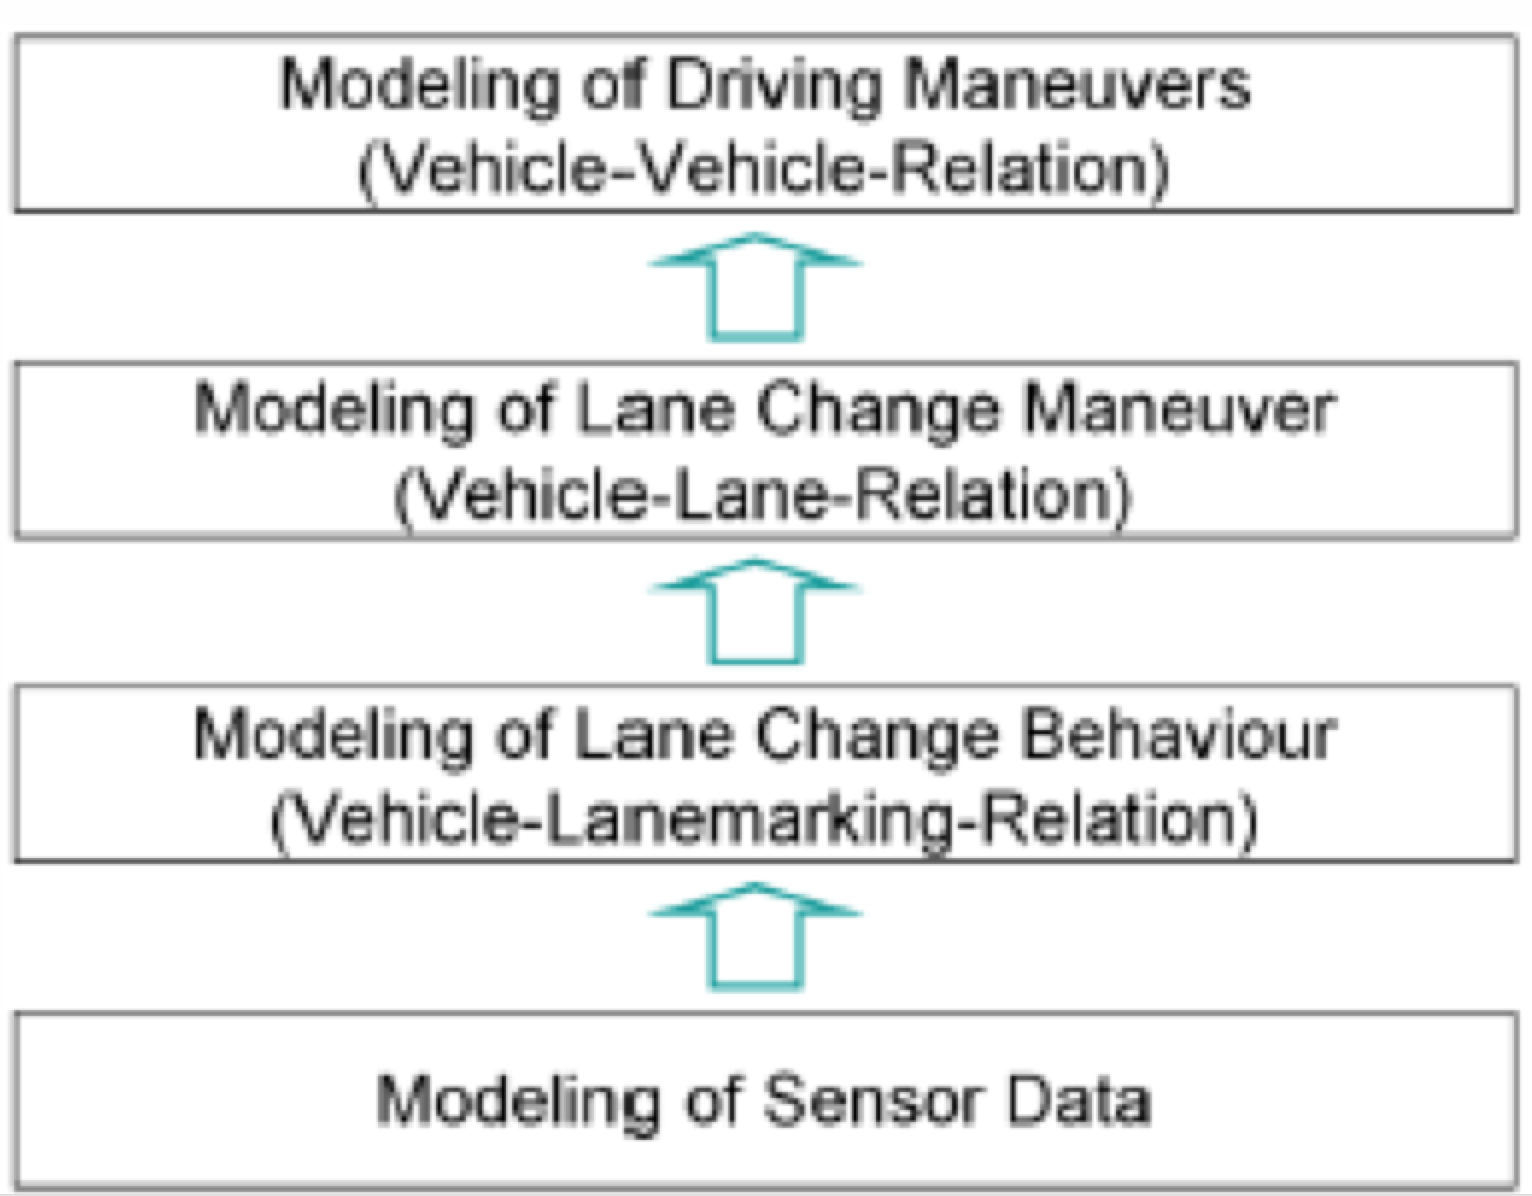
\includegraphics[scale=0.58]{./figures/DaimlerHierarchicalModelling}
\caption{\label{Figure:DaimlerHierarchicalModelling} Hierarchical layers for the recognition of driving manoeuvres.}
\end{center}
\end{figure}

The sensor data is modelled in the first step. Using this layer, a new layer is created on top with the goal of detecting a lane change behaviour. The detection of a lane change behaviour allows the system to model the lane change manoeuvre in a higher layer. Finally, with this information, the system is able to identify the kind of driving manoeuvre which is taking place between a pair of vehicles. 



\subsubsection*{The static-OOBN model}

As commented above, this model will work with the so-called ``object data''. This data mainly consists of a set of measured and/or computed signals or situation-features denoted by $S$ (e.g.. EGO speed, EGO lateral velocity, speed of a car in-front, etc., see \cite{kasper2012object} for further details) describing the traffic scene. The whole modelling is structured in hierarchical layers as detailed in Figure \ref{Figure:DaimlerHierarchicalModelling} and it has been previously implemented \cite{kasper2012object} using an object-oriented Bayesian network (OOBN) \cite{koller1997object}. 


%Even using this high-level features, the modelling problem is very complex. 

%At the same time, the problem contain a lot of structure and can be divided in simpler and similar sub-problems. For example, when deciding whether there is evidence or not that a car is performing a %lateral movement to the right, we can employ two situation-features such as the lateral velocity to the right and the lateral offset w.r.t. the right lane marking of this vehicle to make this decision. But %we will find a quite similar problem when deciding about the lateral movement evidence of the EGO car or any other car, when the only difference that will use another situation-features (e.g. the right %lateral velocity of the EGO) .

The general structure of this OOBN model consists of a number of abstraction levels (see Figure \ref{Figure:DaimlerOOBNAbstraction}): all measured and/or computed signals S\_MEAS are handled with their uncertainties S\_SIGMA. These are represented as object classes at the lowest level (class $S$) of the OOBN. The real values S\_REAL of evidence signals are then used at the next level of the hierarchy to evaluate the hypotheses (class $H$ in Figure \ref{Figure:DaimlerOOBNAbstraction}). The combined evaluation of several hypotheses results in the prediction of events, class E. In our case, the events are modelling traffic manoeuvres of the own and neighbour vehicles.

\begin{figure}
\begin{center}
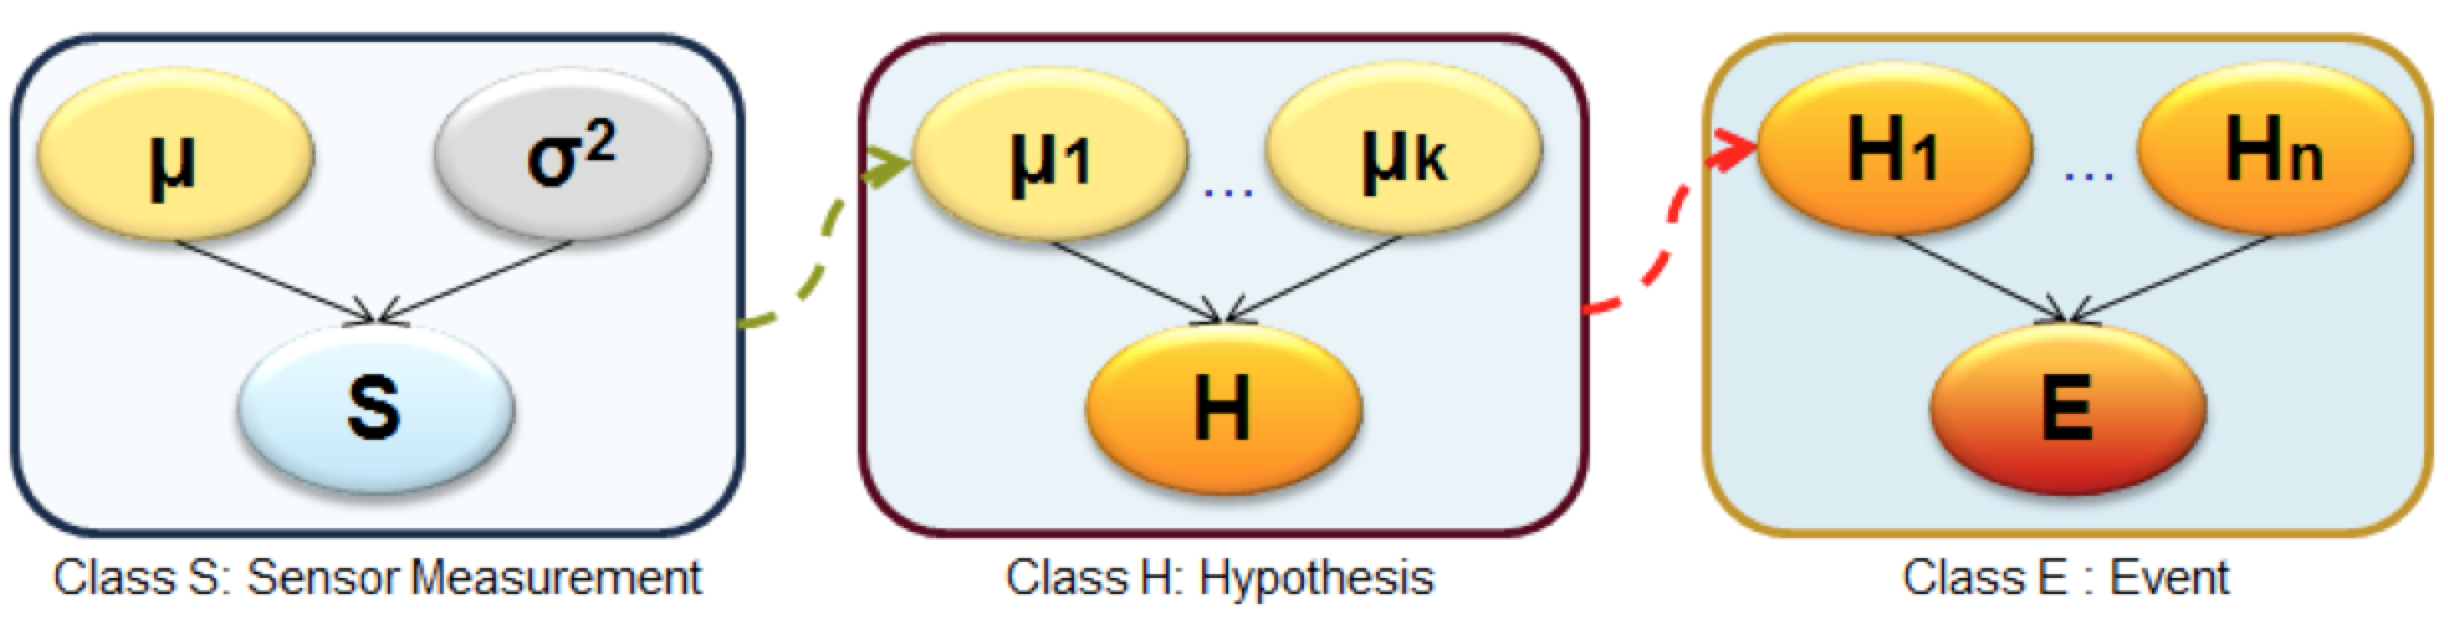
\includegraphics[scale=0.58]{./figures/DaimlerOOBNAbstraction}
\caption{\label{Figure:DaimlerOOBNAbstraction} Static-OOBN model for the prediction of an event (maneuver) \cite{Weidl2014}.}
\end{center}
\end{figure}

As commented above, the observations characterising a situation are acquired from sensors and computations (see Figure \ref{Figure:DaimlerDataFlow}) and, in consequence, they are regarded as  \textit{measured data}. If the measurement instrument is not functioning properly (due to sensor noise or fault), then the sensor-reading (S\_MEAS) and the real variable (S\_REAL) under measurement need not to be the same. This fact imposes the causal model structure as shown in the first part on Figure \ref{Figure:DaimlerOOBNAbstraction}. The sensor-reading of any measured variable is conditionally dependent on random changes in two variables: real value under measurement (S\_REAL) and sensor fault (S\_SIGMA).

The situation features used for manoeuvre recognition are structured along three main dimensions: lateral evidence (LE), trajectory (TRAJ), and occupancy schedule grid (OCCGRID). They represent the three hypotheses (see Figure \ref{Figure:DaimlerOOBNAbstraction}), which are modelled by the corresponding OOBN-fragments \cite{kasper2012object}. The BN fragment for the hypothesis LE is shown in Figure \ref{Figure:DaimlerLE}. Its conditional probability distribution is represented by a sigmoid (logistic) function. This is used to model the growing probability for the lateral evidence to cross the lane marking, based on the vehicle coming closer to the lane marking (modelled by O\_LAT\_MEAS) and the increase of its lateral velocity (modelled by V\_LAT\_ MEAS).

\begin{figure}
\begin{center}
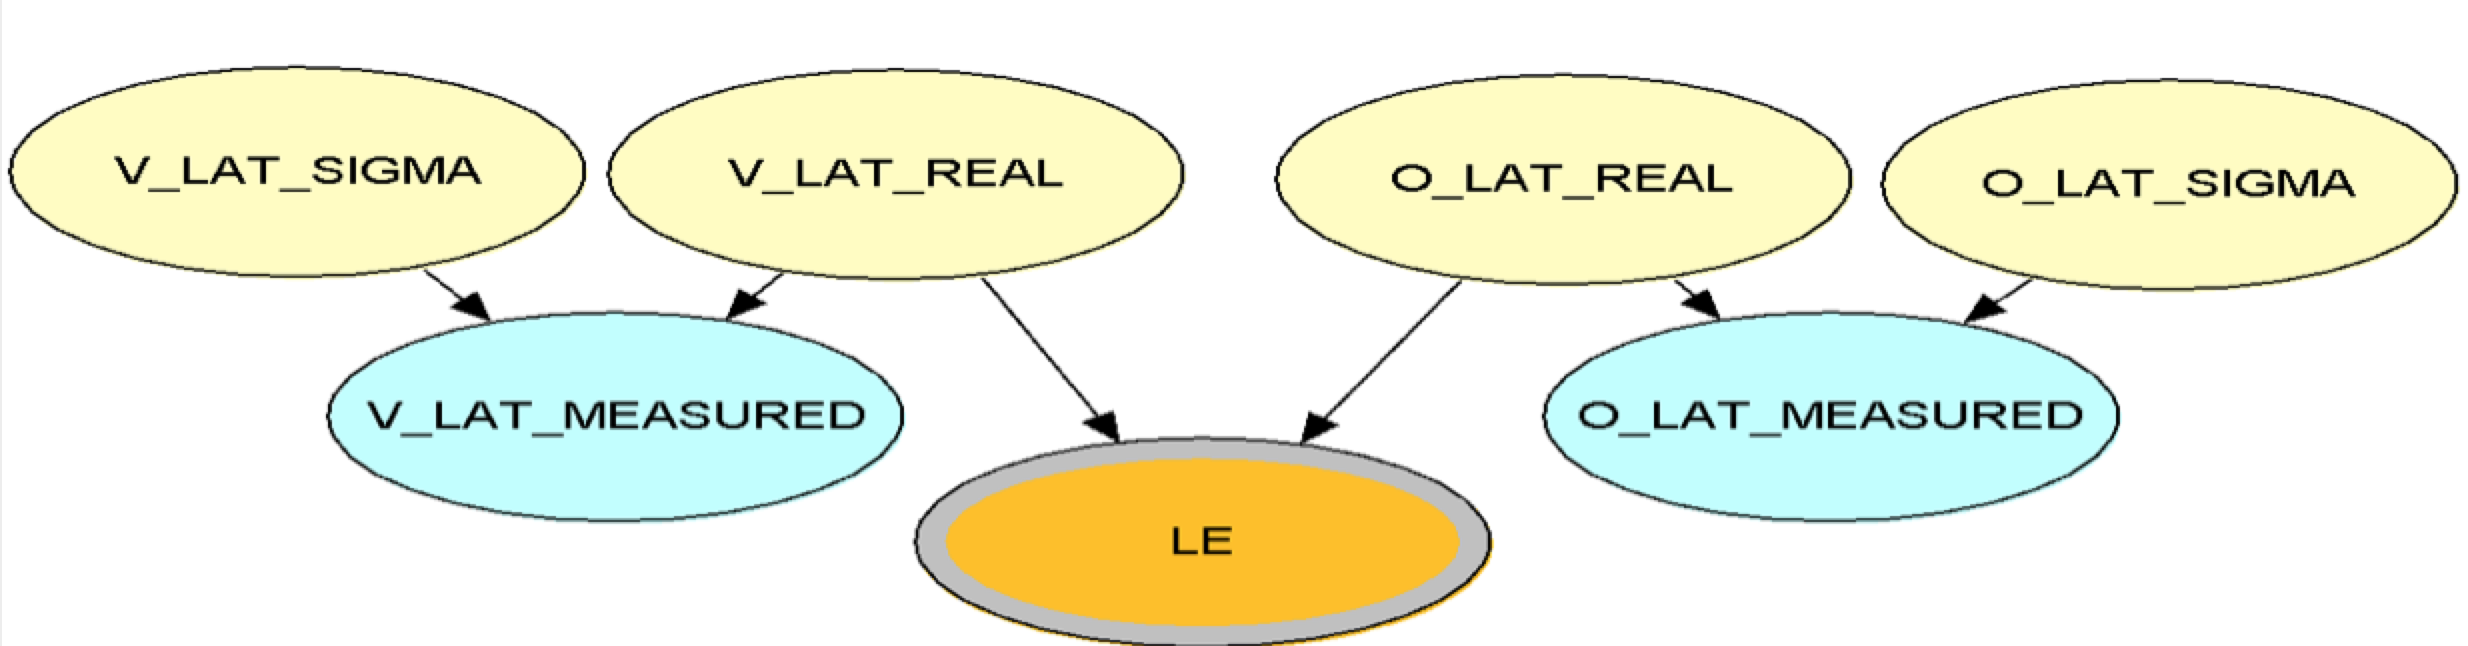
\includegraphics[scale=0.58]{./figures/DaimlerLE}
\caption{\label{Figure:DaimlerLE} Static BN fragment for the LE hypothesis.}
\end{center}
\end{figure}

The right-hand square on Figure \ref{Figure:DaimlerOOBNAbstraction} abstractly shows how these hypotheses are combined into events, which in our automotive scenario correspond to the different driving manoeuvres: lane follow, lane change (cut-in, cut-out), expressed for ego and surrounding objects\cite{kasper2012object}.

\subsubsection*{The dynamic-OOBN model}

The above described static OOBN is able to detect a manoeuvre 0.6s before execution. As detailed in the DoW [], the goal is to extend the prediction horizon for manoeuvre recognition at least to 1-2 seconds (max. 4-5 seconds ahead) before the actual lane marking crossing, which is of advantage for the adaptive cruise control. Moreover, this early detection of the manoeuvre should be at not expenses of the prediction accuracy,  as indicated on Daimler's use cases \cite{Fer14}, the area under the ROC curve (AUC) should be greater than 0.96 for 1 second and greater than 0.9 for 2 seconds.

Figure \ref{Figure:daimlerTPlot} shows an example of the current performance, and limitations, of the static-OOBN model. In these figures we plot the evolution on different time-steps for lateral velocity and lateral offset to a lane marking in an ongoing Object-CutOut and Object-Cutin manoeuvres (see Figure \ref{Figure:DaimlerManeuvers}). The vertical black bar in these figures indicates the moment in which the manoeuvre has been recognised by the static-OOBN. The manoeuvre is finished at the end of the series, which coincides with the actual moment of changed lane. The black line corresponds to the lateral offset and lateral velocity of the EGO car, which is just following the lane (LF), and the green line to the values of the Object car performing the Object-CutOut/Object-Cutin manoeuvres. As expected for lane follow (LF), the lateral velocity of the EGO fluctuates around zero  (i.e. EGO car is just driving inside its lane) and the lateral offset of the lane marking is almost constant all the time. However, when we look at the lane change behaviour of the OBJ car (green lines) we easily see a quite different behaviour. Firstly, we observe that the lateral velocity is much  higher indicating a lateral movement. Similarly, we also observe how the lateral offset steadily increases, what clearly indicates that the Object car is leaving its current lane in both manoeuvres. 

\begin{figure}
\begin{center}
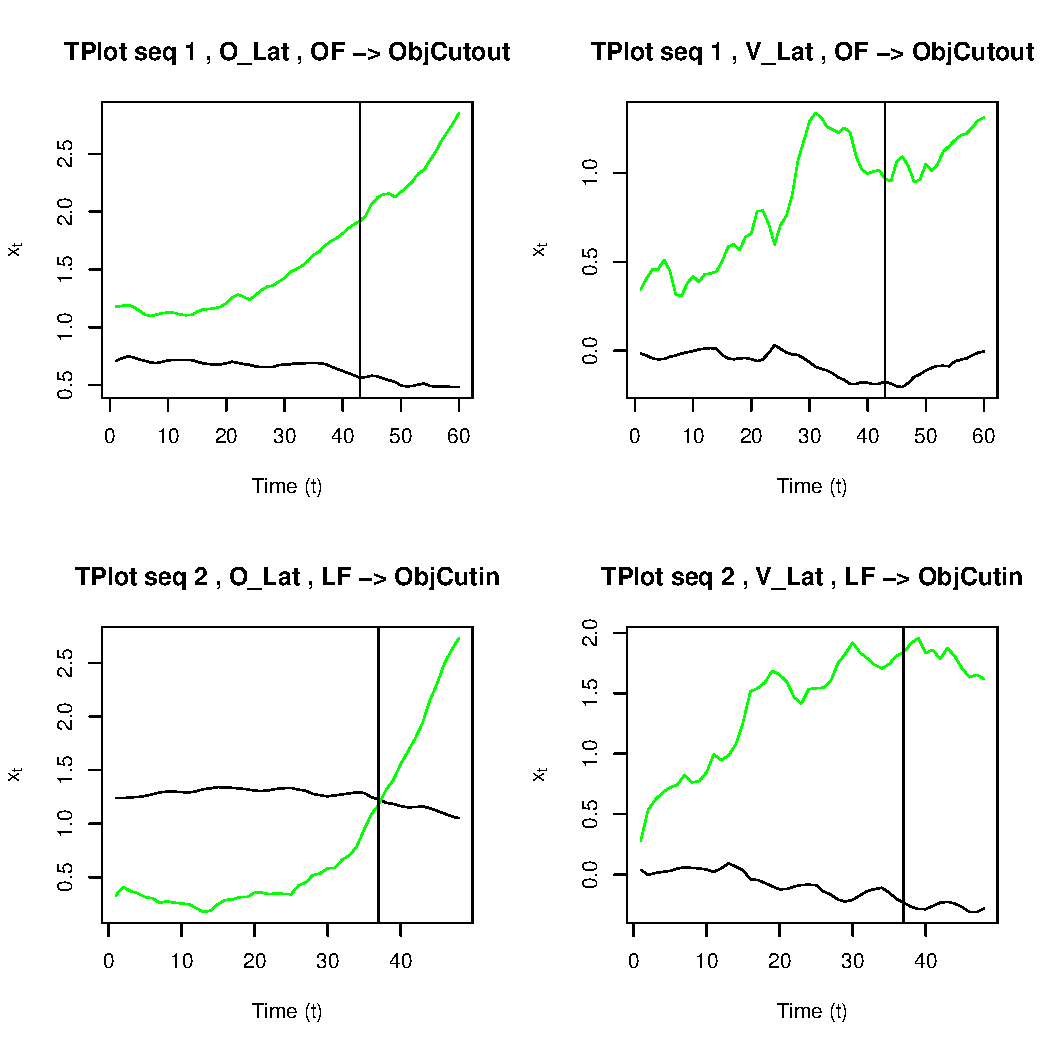
\includegraphics[scale=0.65]{./figures/DaimlerLE_EGO_L_LE_OBJ_L_OBJCut.pdf}
\caption{\label{Figure:daimlerTPlot}Daimler Time Plot}
\end{center}
\end{figure}

the 

Although the manoeuvre is clearly identified before it completes in both cases (approx. 0.6 seconds in advance), it is desired to predict it 1-2 seconds in advance. Looking at the evolution of lateral offset and velocity in Figure \ref{Figure:daimlerTPlot}, we could argue that the detection of the manoeuvre can be performed earlier (i.e. when the lateral offset and lateral velocity starts to increases consistently). This is one of the basic piece of evidence that motivated the development of the dynamical version of the static-OOBN model \cite{Weidl2014}.  Another piece of evidence comes when we look at sample correlograms for lateral velocity and offset (that is, the correlation of the data with lagged values of themselfves) plotted in Figure \ref{Figure:daimlerCorrel}. There we can see as there is a strong temporal dependency (the correlation coefficients are high) for the two variables when we consider not many time steps between the temporal observations. So, the employment of a dynamic model to make predictions about the evolution of the lateral velocity and lateral offset in a near future seems to be reasonable with this analysis. So, our main assumption is that the use of dynamic Bayesian network models (see Section \ref{Section:Preliminaries}) will allow us to build a more accurate and reliable system for manoeuvre recognition. 

\begin{figure}
  \centering
    \begin{tabular}{cc}
    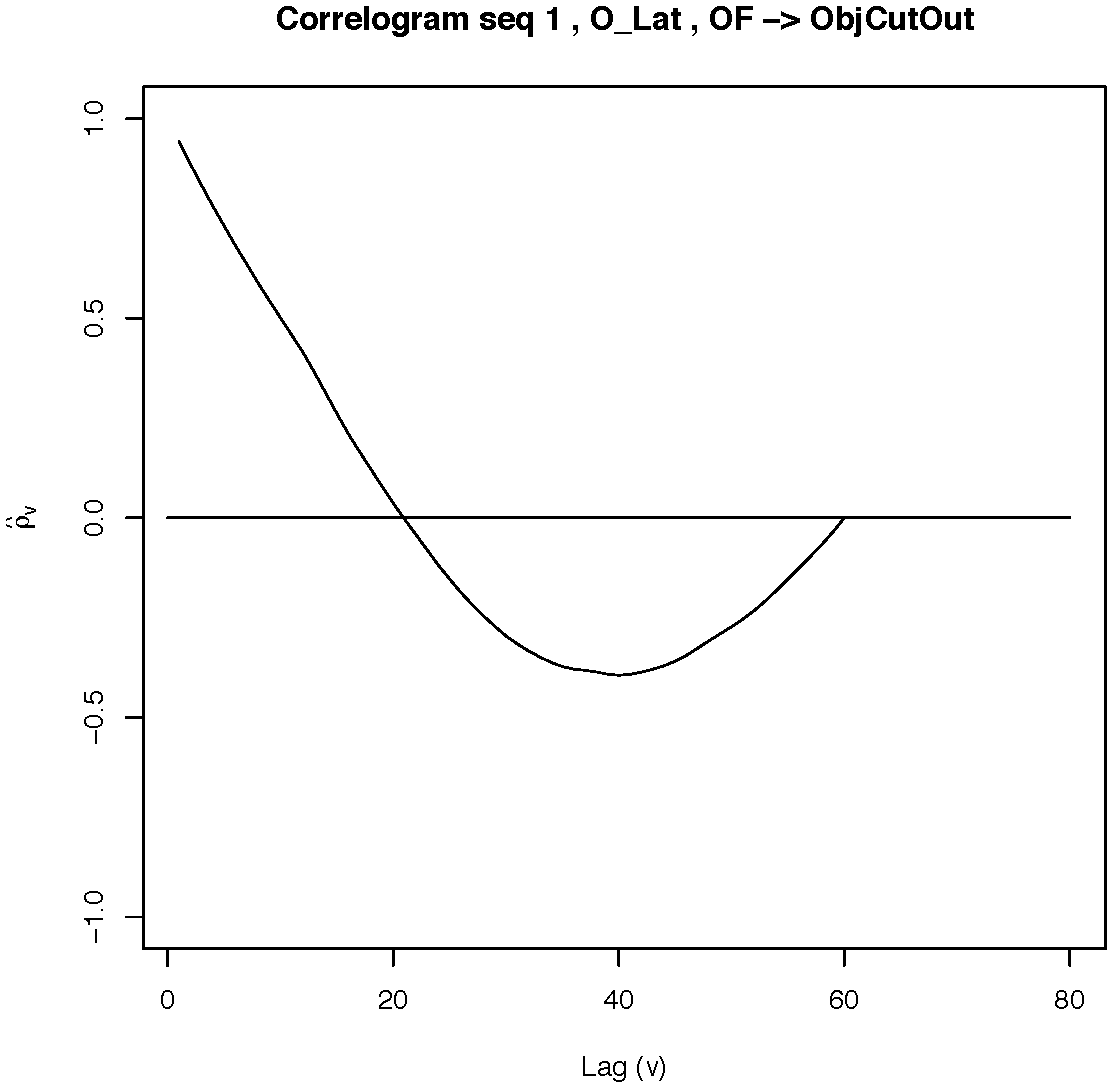
\includegraphics[width=60mm]{figures/DaimlerCorrOBJ_R80Offs.pdf}&
    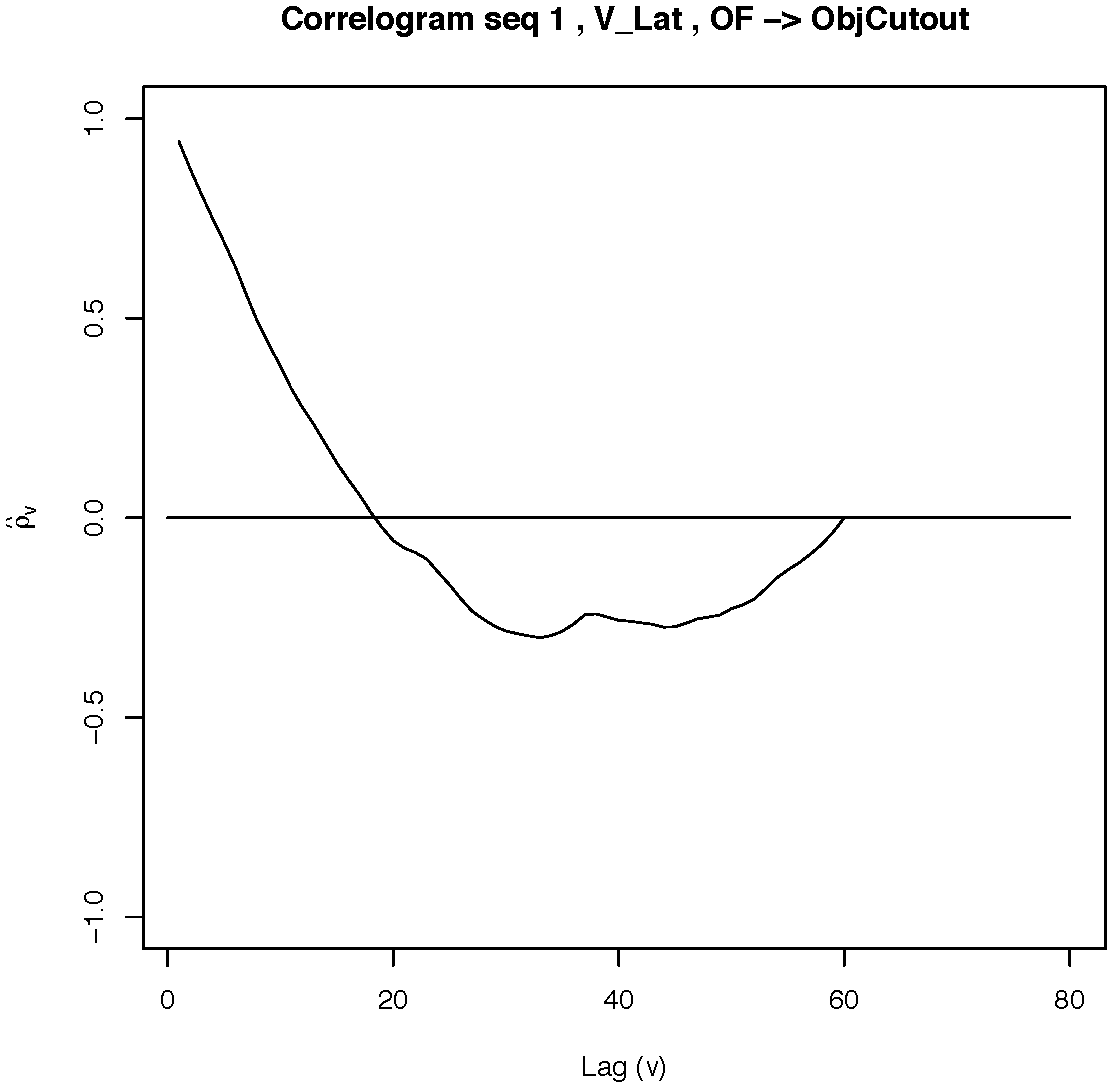
\includegraphics[width=60mm]{figures/DaimlerCorrOBJ_R80Vel.pdf}\\
  \end{tabular}
    \caption{\label{Figure:daimlerCorrel}Correlograms for Lateral velocity and offset.}
\end{figure}

In any case, let us note however that the prediction horizon for manoeuvre recognition is going to be limited in order to avoid false positives (i.e. recognizing a lane change manoeuvre when the driver was just performing some random lateral movement).  In case of a false positive, such as an erroneously Object-CutIn for instance, the adaptive cruise control would react with an unnecessary break, so they ought to be avoided.

\begin{figure}
\begin{center}
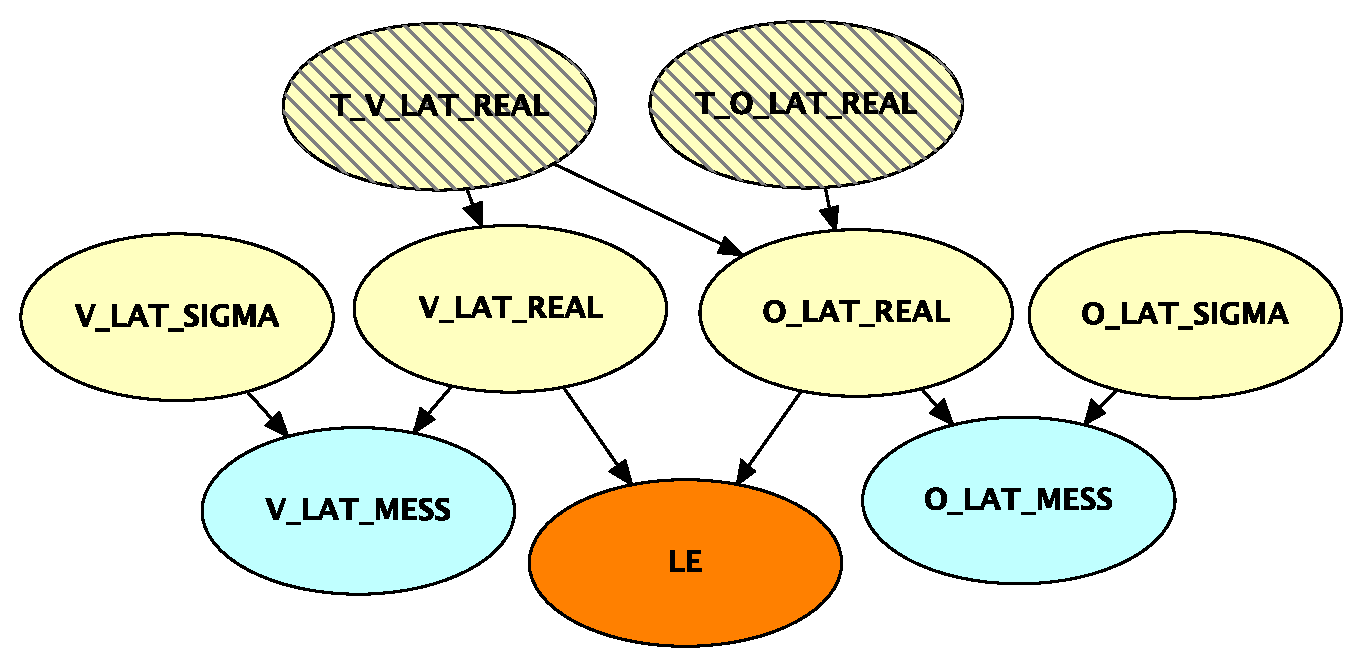
\includegraphics[scale=0.58]{./figures/DaimlerLEdyn}
\end{center}
\caption{\label{Figure:daimlerLEdyn}Daimler Temporal fragment for the LE hypothesis.}
\end{figure}

As explained in Section \ref{Section:Preliminaries}, the dynamic extension involves copies of the static OOBN for different number of time steps in the time window. Fig. \ref{Figure:daimlerLEdyn} shows an example for the LE hypothesis, where the two top nodes are temporal clones defining the share belief state between consecutive time steps, and hence creating a first order Markov process. This one the model proposed in \cite{Weidl2014} by some of the AMIDST partners.  The first order assumption is a standard assumption in this kind of models and helps to simplify the posterior inference and learning process. Fortunately, if we build a partial-correlogram as the ones plotted in Figure \ref{Figure:daimlerPartialCorrel}, we can see that this assumptions seems to reasonable because the influence of $O\_LAT_{t-2}$ on $O\_LAT_{t}$ given $O\_LAT_{t-1}$ is close to null (i.e. the value at $v=2$ is close to null in Figure \ref{Figure:daimlerPartialCorrel}). Same applies to $V\_LAT$.

\begin{figure}
  \centering
    \begin{tabular}{cc}
        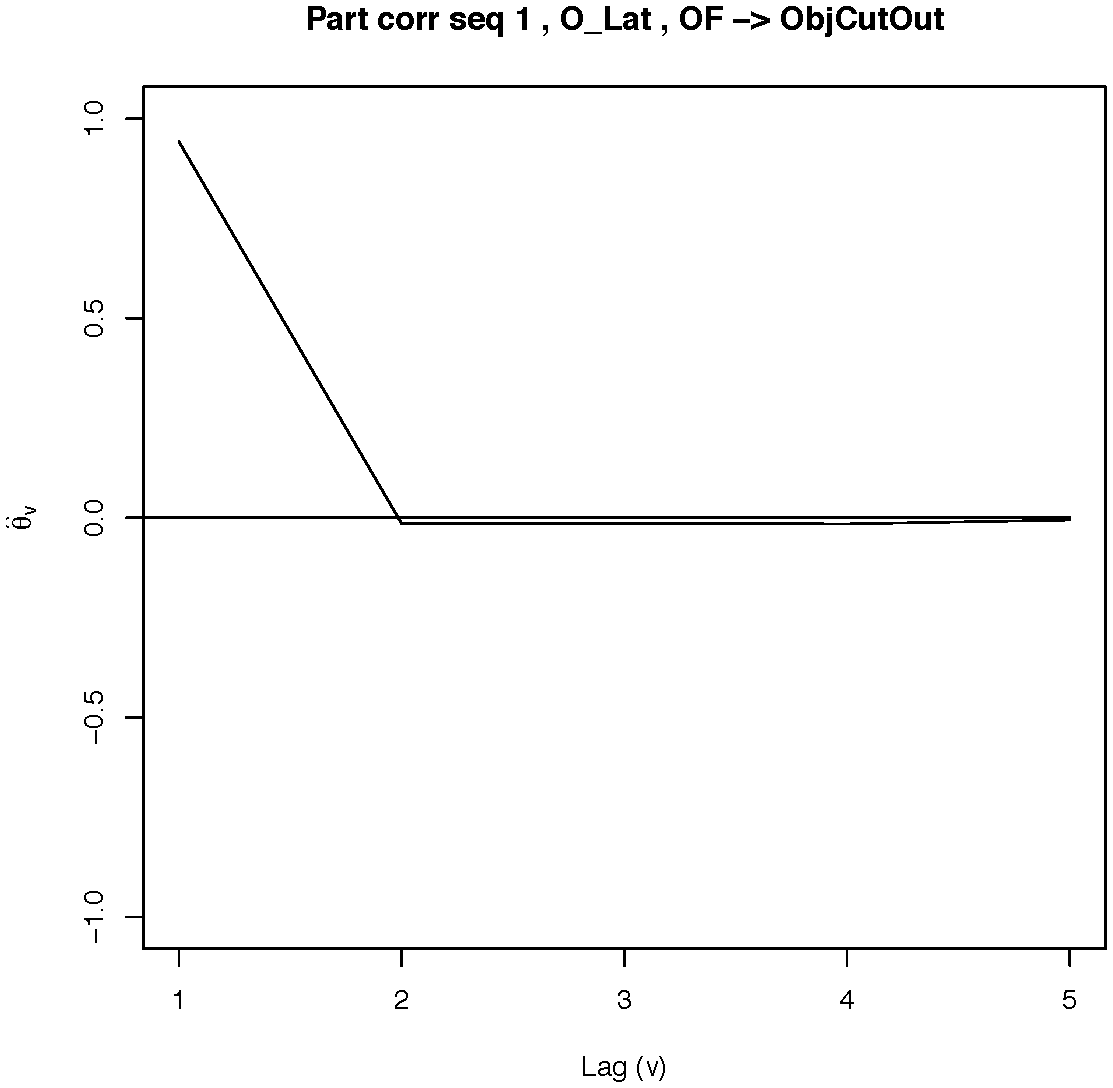
\includegraphics[width=60mm]{figures/DaimlerPcorrOBJ_R5Offs.pdf}&
    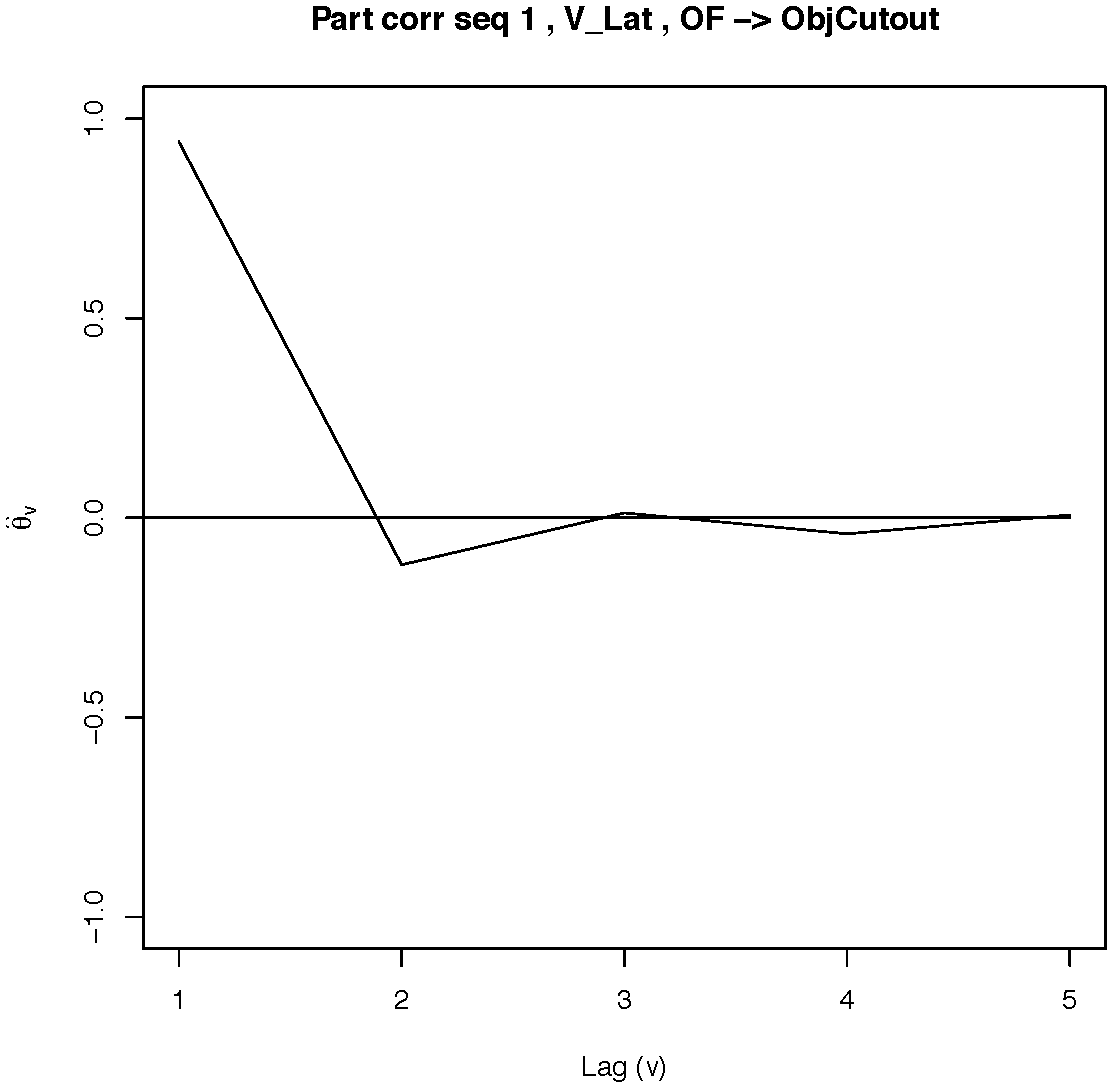
\includegraphics[width=60mm]{figures/DaimlerPcorrOBJ_R5Vel.pdf}\\
  \end{tabular}
    \caption{\label{Figure:daimlerPartialCorrel}Partial-Correlograms for Lateral velocity and offset.}
\end{figure}


As described in \cite{Weidl2014}, the proposed dynamic BN (DBN) aimed to incorporate the trend of change for the real values, where their physics relations are represented as causal dependencies between the time steps $dt$, e.g. in Fig. \ref{Figure:daimlerLEdyn} the transition function of O\_LAT at time $t$, $O(t)$, is modeled as a Gaussian distribution. Its mean is affected by $O(t-1)$, and by V\_LAT at time $t-1$, $v(t-1)$:

\begin{equation}
O(t) =O(t-1) +v(t-1)dt +N
\end{equation}

where $N$ denotes a white noise $N(0,\sigma^2)$ which is assumed to be small. In order to corroborate the validity of this distributional assumption, we also analysed the hypothesis $O(t) - O(t-1) = \Delta O = v(t-1)dt +N$ on our data. Figure \ref{Figure:daimlerVvsOffs} shows the plot and contour plots for $v$ and $\Delta O$, which show that the assumption of linear relationship with Gaussian noise might not be very far from reality. 

\begin{figure}
  \centering
  \setlength{\tabcolsep}{0.05pt}
  \renewcommand{\arraystretch}{0.02}
    \begin{tabular}{cc}
    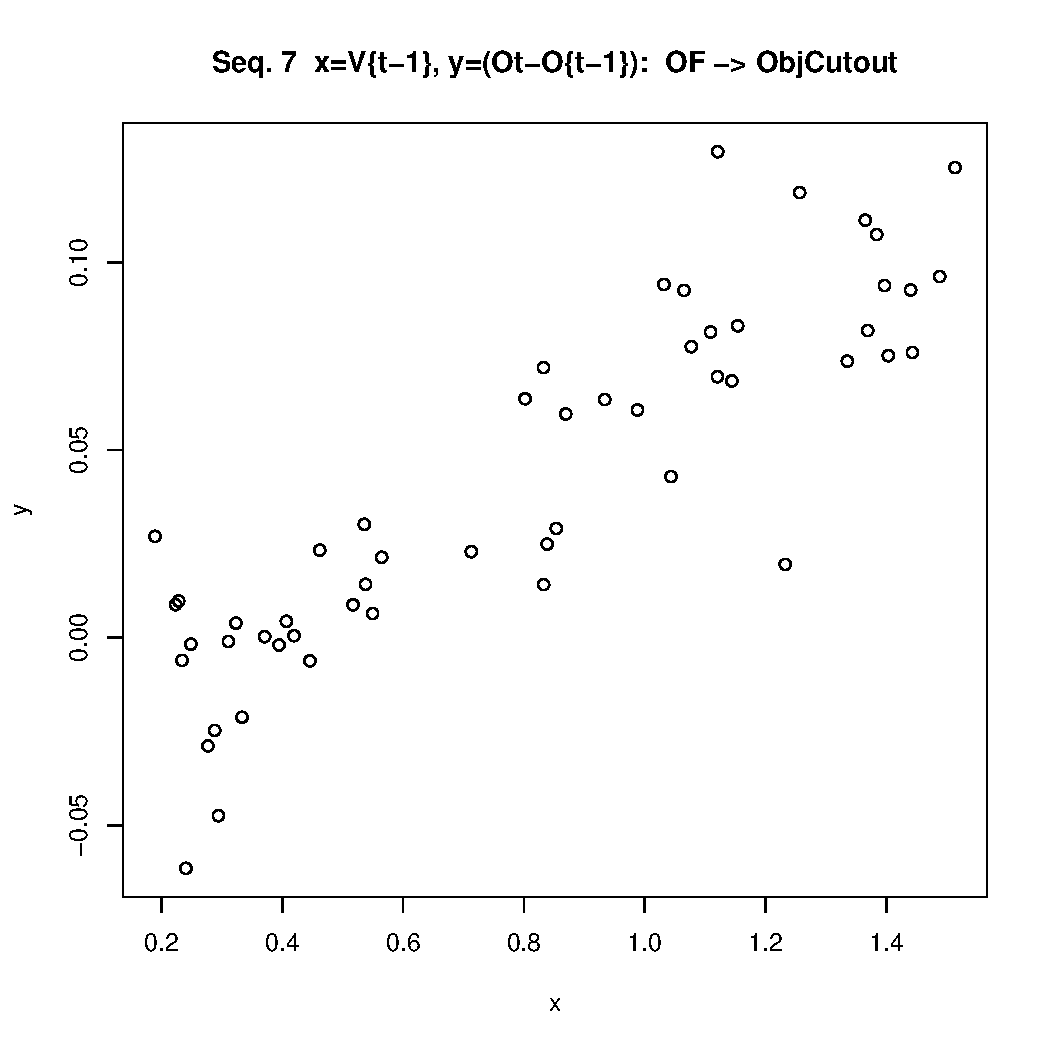
\includegraphics[width=60mm]{figures/DaimlerOBJplotSerie7.pdf}&
    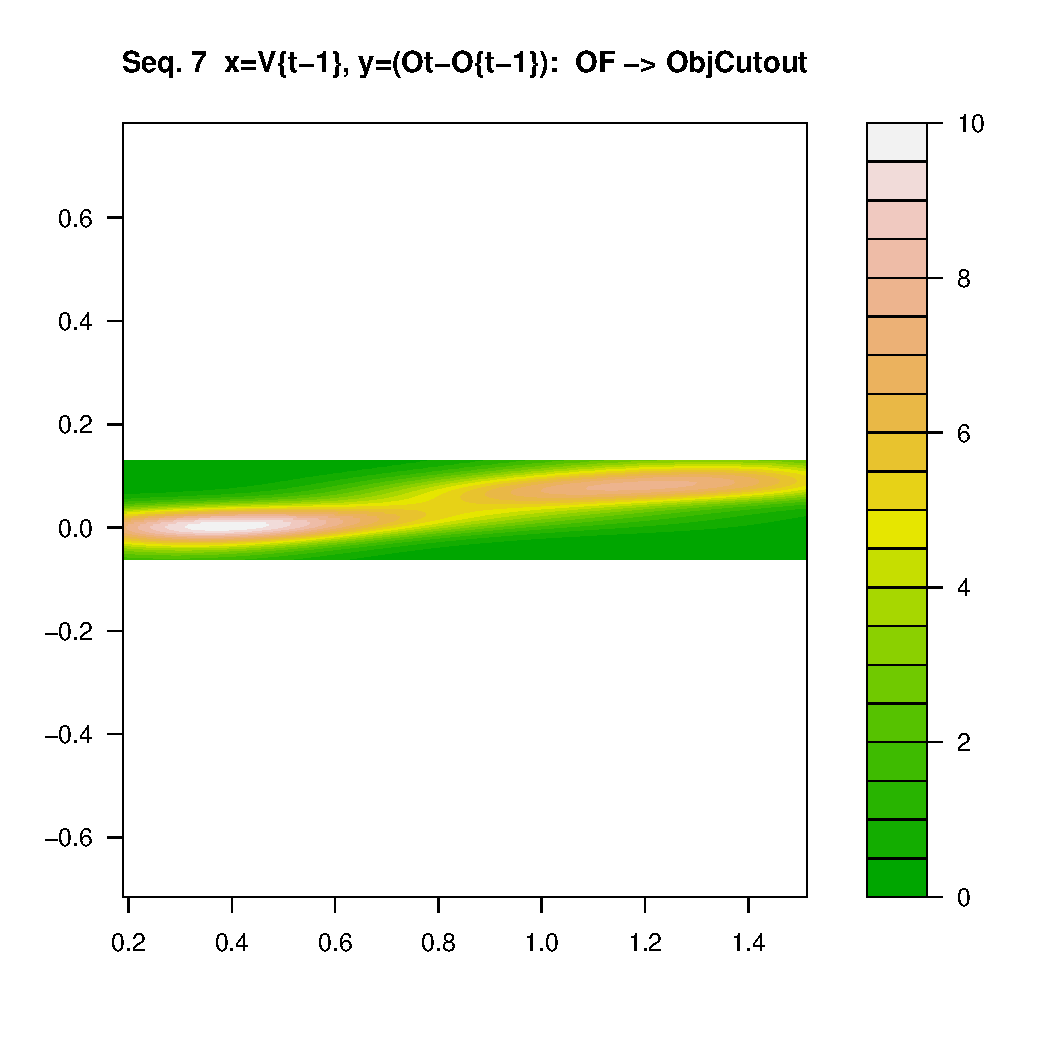
\includegraphics[width=60mm]{figures/DaimlerOBJcontourSerie7.pdf}\\
  \end{tabular}
      \caption{ \label{Figure:daimlerVvsOffs}Time plot for $v(t-1)$ vs $O(t) - O(t-1)$. Linear correlation can be observed.}
\end{figure}

Additionally,  we believe that even earlier prediction of manoeuvre intentions could be achieved before any development of the trend for lateral evidence LE has been observed. A first indication of possible lane change intention can be observed through the relative dynamics between one vehicle (host or object) and the vehicles in front of it on the same lane. Once again, the goal is to further increase the prediction horizon for manoeuvre recognition (up to 5 seconds), and this approach will be further explored in future stages of the project. 

Finally, in Figure \ref{Figure:daimlerLEdynGeneric} we show a rough overview of the final structure of this dynamic Bayesian network\footnote{Full details can not be given for confidentiality reasons}, which shows how the temporal connection is only made on the top nodes involving the situation-features in consecutive time steps.  The final event or manoeuvre prediction is then determined by the combination of these hypotheses and the position of the OBJ with respect to the EGO car.

\begin{figure}
\begin{center}
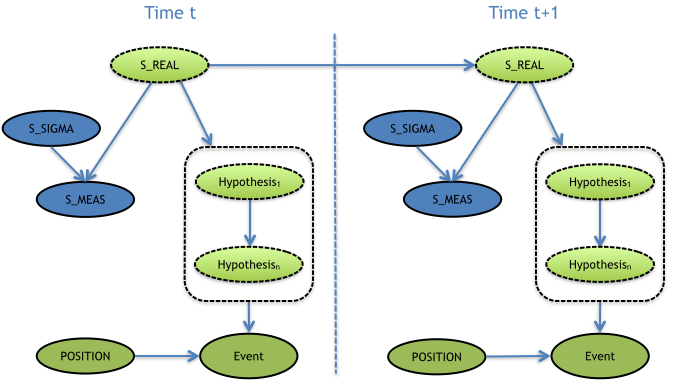
\includegraphics[scale=0.58]{./figures/DaimlerLEdynGeneric}
\end{center}
\caption{\label{Figure:daimlerLEdynGeneric}Daimler Temporal model with several hypothesis.}
\end{figure}



%A DBN induces a number of constraints on the compilation of the network into a computational structure. One constraint relates to transferring the belief state from one time slice to the next where the belief state is the probability distribution over the variables shared by neighbouring time slices. In general, the belief state is transferred as a joint distribution. We have imposed limitations in our dynamic model so that the next state depends only on the current state, and not on the sequence of events that preceded it, i.e. first order Markov model. Although in principle this might seem as a strong limitation, we have reasons to believe that this property might hold in our data. Fig. \ref{Figure:daimlerCorrel} displays, at the top, the sample correlograms for lateral velocity and offset, that is, the correlation of the data with lagged values of themselfves. The partial correlogram (bottom figures) is used to remove the common linear effect of the data in between samples. In our example, for both variables, the correolograms take some time to decay to zero, while the partial correlograms are large for lag one and then small of all other lags. This indicates that the correlation between non consecutive samples is due to the common relationship of these samples and the samples in between \cite{Newton:1988}.


\drop{ %To be included in the next version of the deliverable
\item \textbf{New hypothesis: Relative Dynamics (REL\_DYN)}

Earlier prediction of manoeuvre intentions can be achieved even before any development of the trend for lateral evidence LE has been observed. A first indication of possible lane change intention can be observed through the relative dynamics between one vehicle (host or object) and the vehicles in front of it on the same lane. Once again, the goal is to further increase the prediction horizon for manoeuvre recognition (up to 5 seconds). 

We can include qualitatively new information based on driving experience, which indicates a need for a lane change if a slower vehicle is driving in front of the own vehicle on the same lane. To continue its safe driving, the approaching vehicle should either break and reduce its speed to the speed of the vehicle in front or, alternatively,,it should change to the neighbour lane, if the neighbour lane is free and no other vehicle is approaching with a higher speed than the own vehicle. A continued safe manoeuvre (of type ``lane follow'' or ``lane change'') is modelled by estimating the TTC (TimeToCollision) to the vehicle in front (on the same lane) or to eventually approaching vehicle (on the neighbour lane). For safe manoeuvre, TTC should be bigger than 1 second, if the own vehicle wants to change to the neighbour lane or if it needs to break to ensure safe driving on the same lane (``'lane follow'') .

Figure [timedetectionRelDyn] shows the evolution on time for the velocity and distance in an EGO\_CutOut manoeuvre. The vertical bar indicates the moment in which the manoeuvre has been recognised by the static OOBN. By taking the temporal properties of the relative dynamics into account on the DBN, we should be able to predict the manoeuvre even earlier on time.

By analogy to Fig. \ref{Figure:daimlerLEdyn}, the original OOBN has been extended with the hypothesis ``relative dynamics'' (REL\_DYN), as shown in Fig.\ref{Figure:daimlerreldyn}. This BN fragment  models the hypothesis REL\_DYN with 3 states Left/Follow/RIGHT, utilising the independency assumption for the discrete variables V\_REL\_MEASSURED and X\_REL\_MEASSURED.

\begin{figure}
\begin{center}
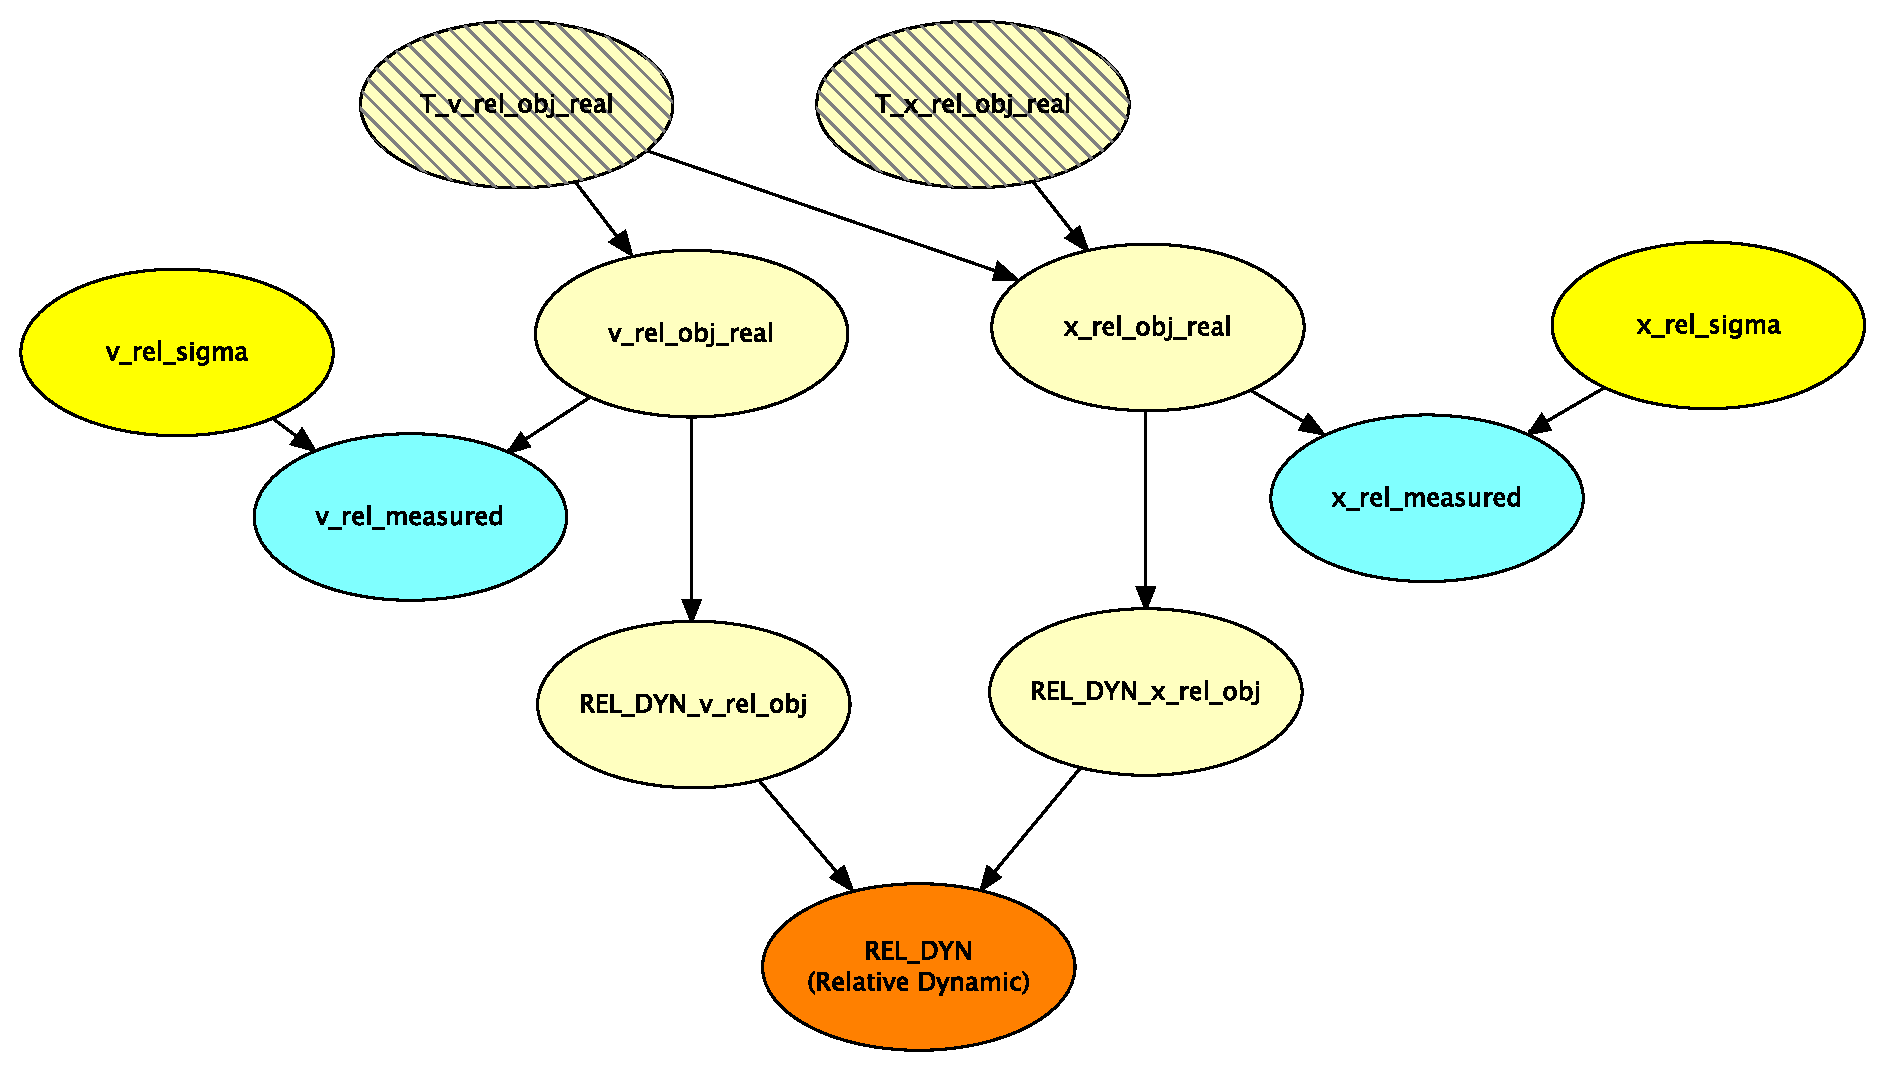
\includegraphics[scale=0.4]{./figures/Daimlerreldyn.pdf}
\end{center}
\caption{\label{Figure:daimlerreldyn}Daimler Temporal Model with relative dynamics}
\end{figure}

If we compare the structure of this network with that of Fig. \ref{Figure:daimlerLEdyn}, we can observe two additional nodes:  REL\_DYN\_V\_REL\_OBJ and REL\_DYN\_X\_REL\_OBJ. They are the results of a modelling trick to simplify the EM-learning of parameters from data for the static BN fragment.

\textcolor{red}{Note that the new REL\_DYN hypothesis introduced would require two instances in the OOBN, one for the relative dynamics of the EGO with the OBJ in front, and another one for the OBJ and another OBJ in front of it. Each REL\_DYN would indicate if the EGO and the OBJ cars are going to turn right, left or continue straight.}
%\end{enumerate}
}

